\section{Design}

\subsection{Node Components}

As the sensor nodes and the repeater are situated outside and rely on solar
power, they required components that were highly power-efficient, while also
being capable of transmitting small data packets via LoRa. An equally important
consideration for the design was how to weatherproof the final enclosure to
protect the sensitive electronics from water ingress and environmental damage.

\subsubsection{Challenger RP2040 LoRa}

The iLabs Challenger RP2040 LoRa (Figure~\ref{fig:challenger-rp2040} )is an
embedded computer that uses the Raspberry Pi RP2040 chip that was released in
2021. The RP2040 itself is a low-cost and power-efficient processor easily
capable of performing the data encoding and transmission in my use case.
Additionally, the chip is extremely popular with over 10 million units being
produced in the first two years of release \cite{pounder2023}. This popularity
means there is ample documentation for developing with this processor.

\begin{figure}[H]
    \centering
    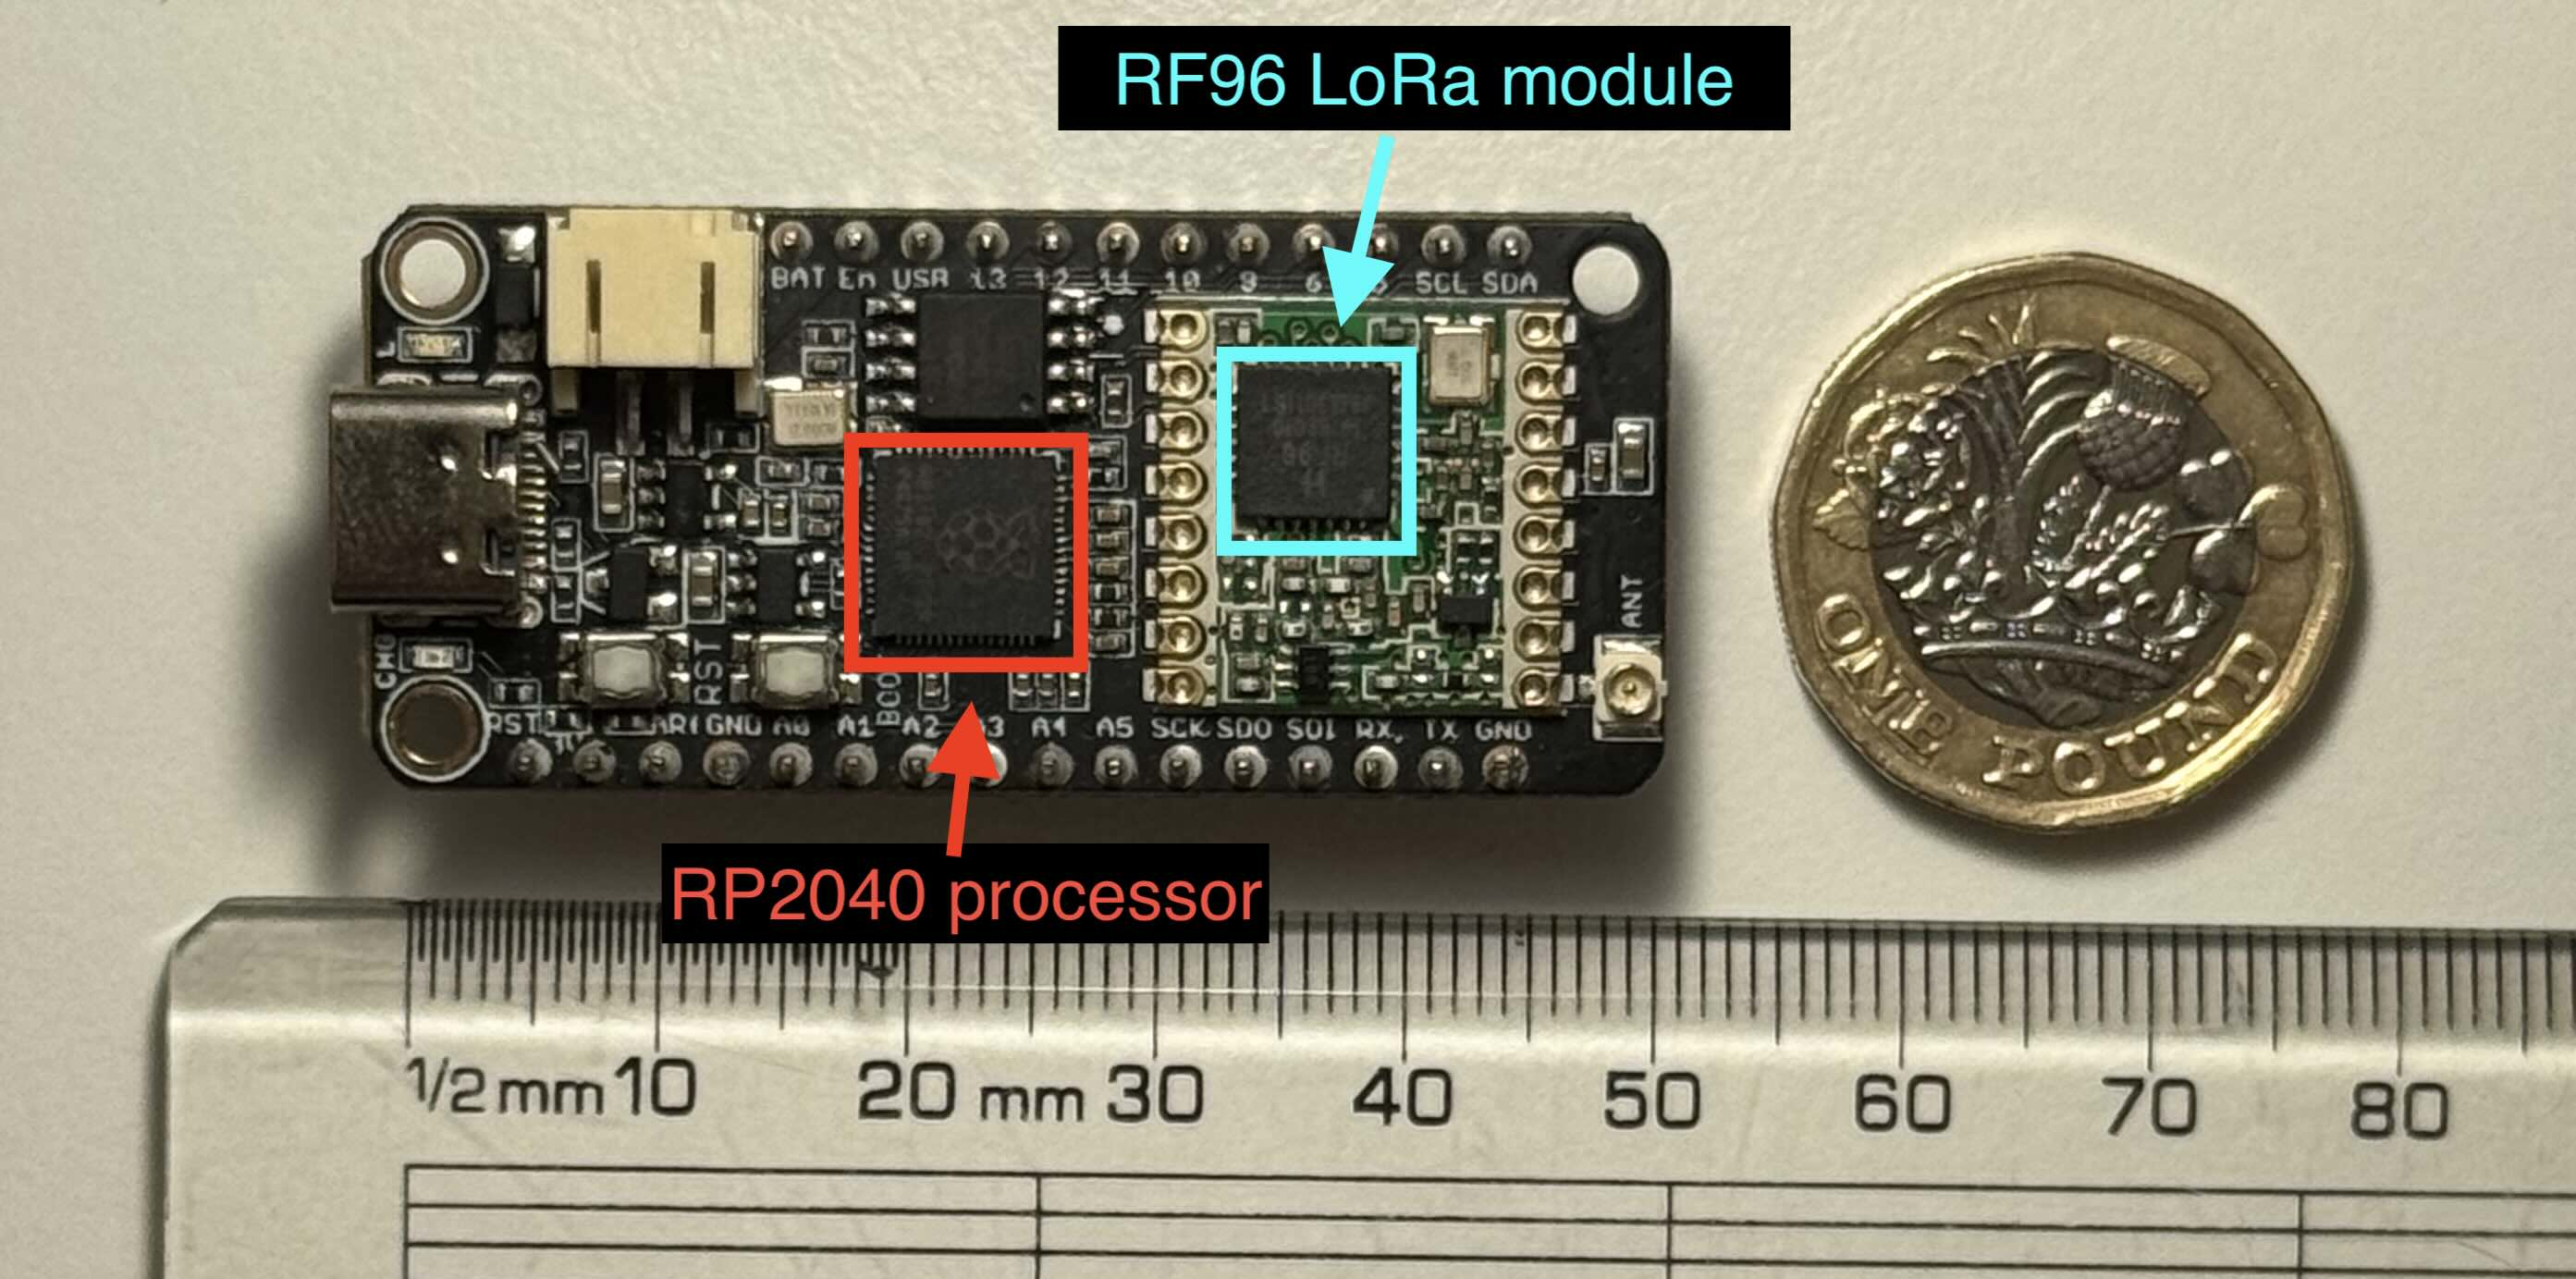
\includegraphics[width=0.8\textwidth]{contents/part-2/fig2/challenger-rp2040.jpg}
    \caption{iLabs Challenger RP2040}
    \label{fig:challenger-rp2040}
\end{figure}

The Challenger board itself is well suited for this project for several reasons.
It uses the compact Adafruit feather form factor, giving a board dimension of
just 5cm by 2cm, making it easy to mount in a small enclosure. The onboard Hope
RF96 LoRa modem is built directly into the board and the U.FL antenna connector
allows for the swapping of antenna's to different varieties. This board's LoRa
module is also set to transmit at a frequency of 868mhz which is a standard UK
frequency for LoRa and gives a good balance between range and bandwidth.

Another useful aspect of the board is the abundance of GPIO pins (20 in total)
allowing for a large number of sensors to be fitted to the board.

\subsubsection{Antennae}

The selection of antennae is one of the largest determinants of range and
reliability in the context of wireless communication systems \cite{khan2016}.
Initially I used a simple PCB antenna as shown in Figure~\ref{fig:pcb-antenna},
however as explained in the next chapter, the range of this was insufficient for
my use.

\begin{figure}[H]
    \centering
    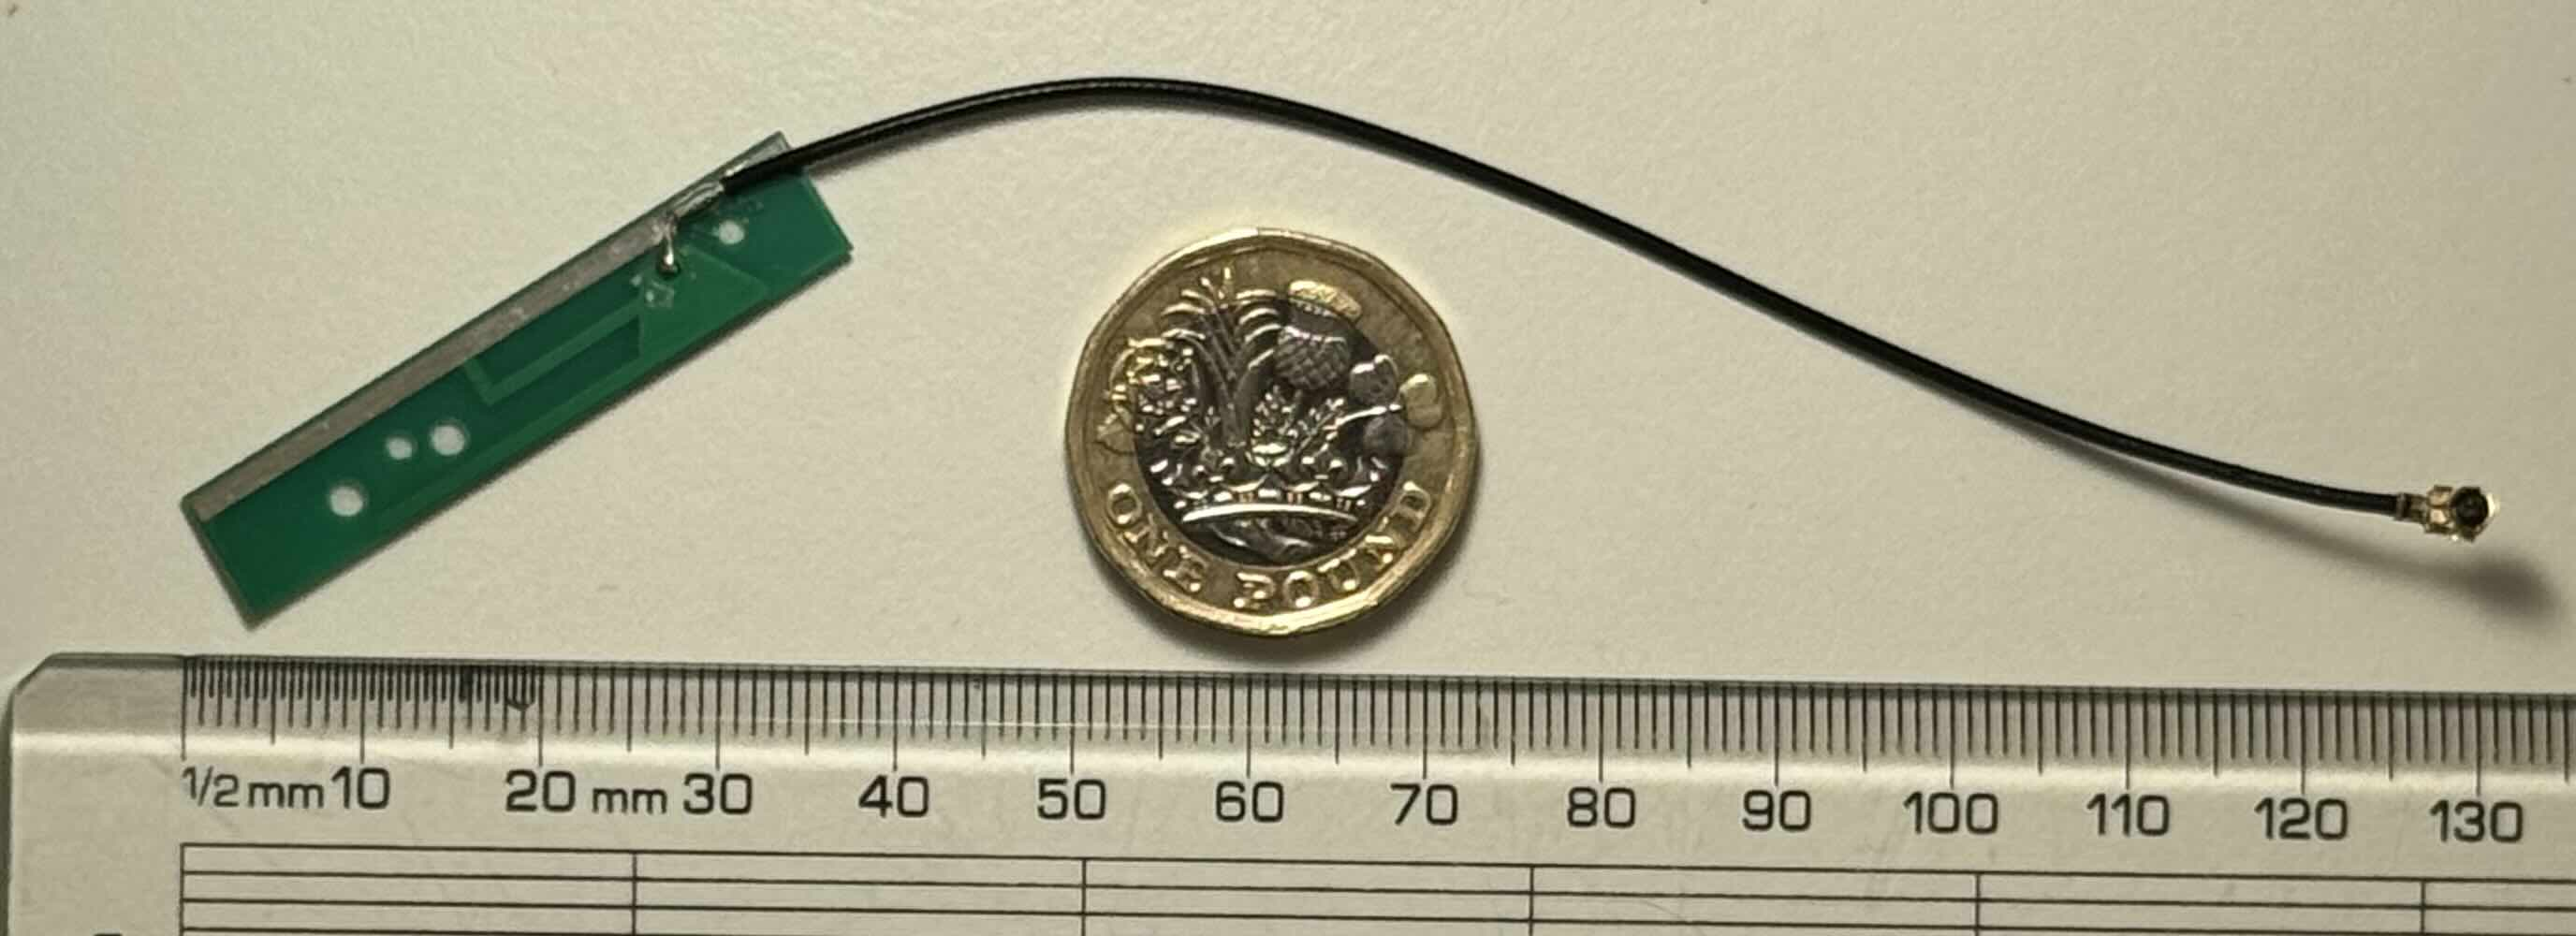
\includegraphics[width=0.8\textwidth]{contents/part-2/fig2/basic-antenna.jpg}
    \caption{Low range PCB antenna}
    \label{fig:pcb-antenna}
\end{figure}

To improve overall range I switched to a more capable omnidirectional whip
antenna that was made specifically for the Challenger RP2040. The antenna is
tuned to perform best at the 868mhz frequency range - which is the range I was
using.

\begin{figure}[H]
    \centering
    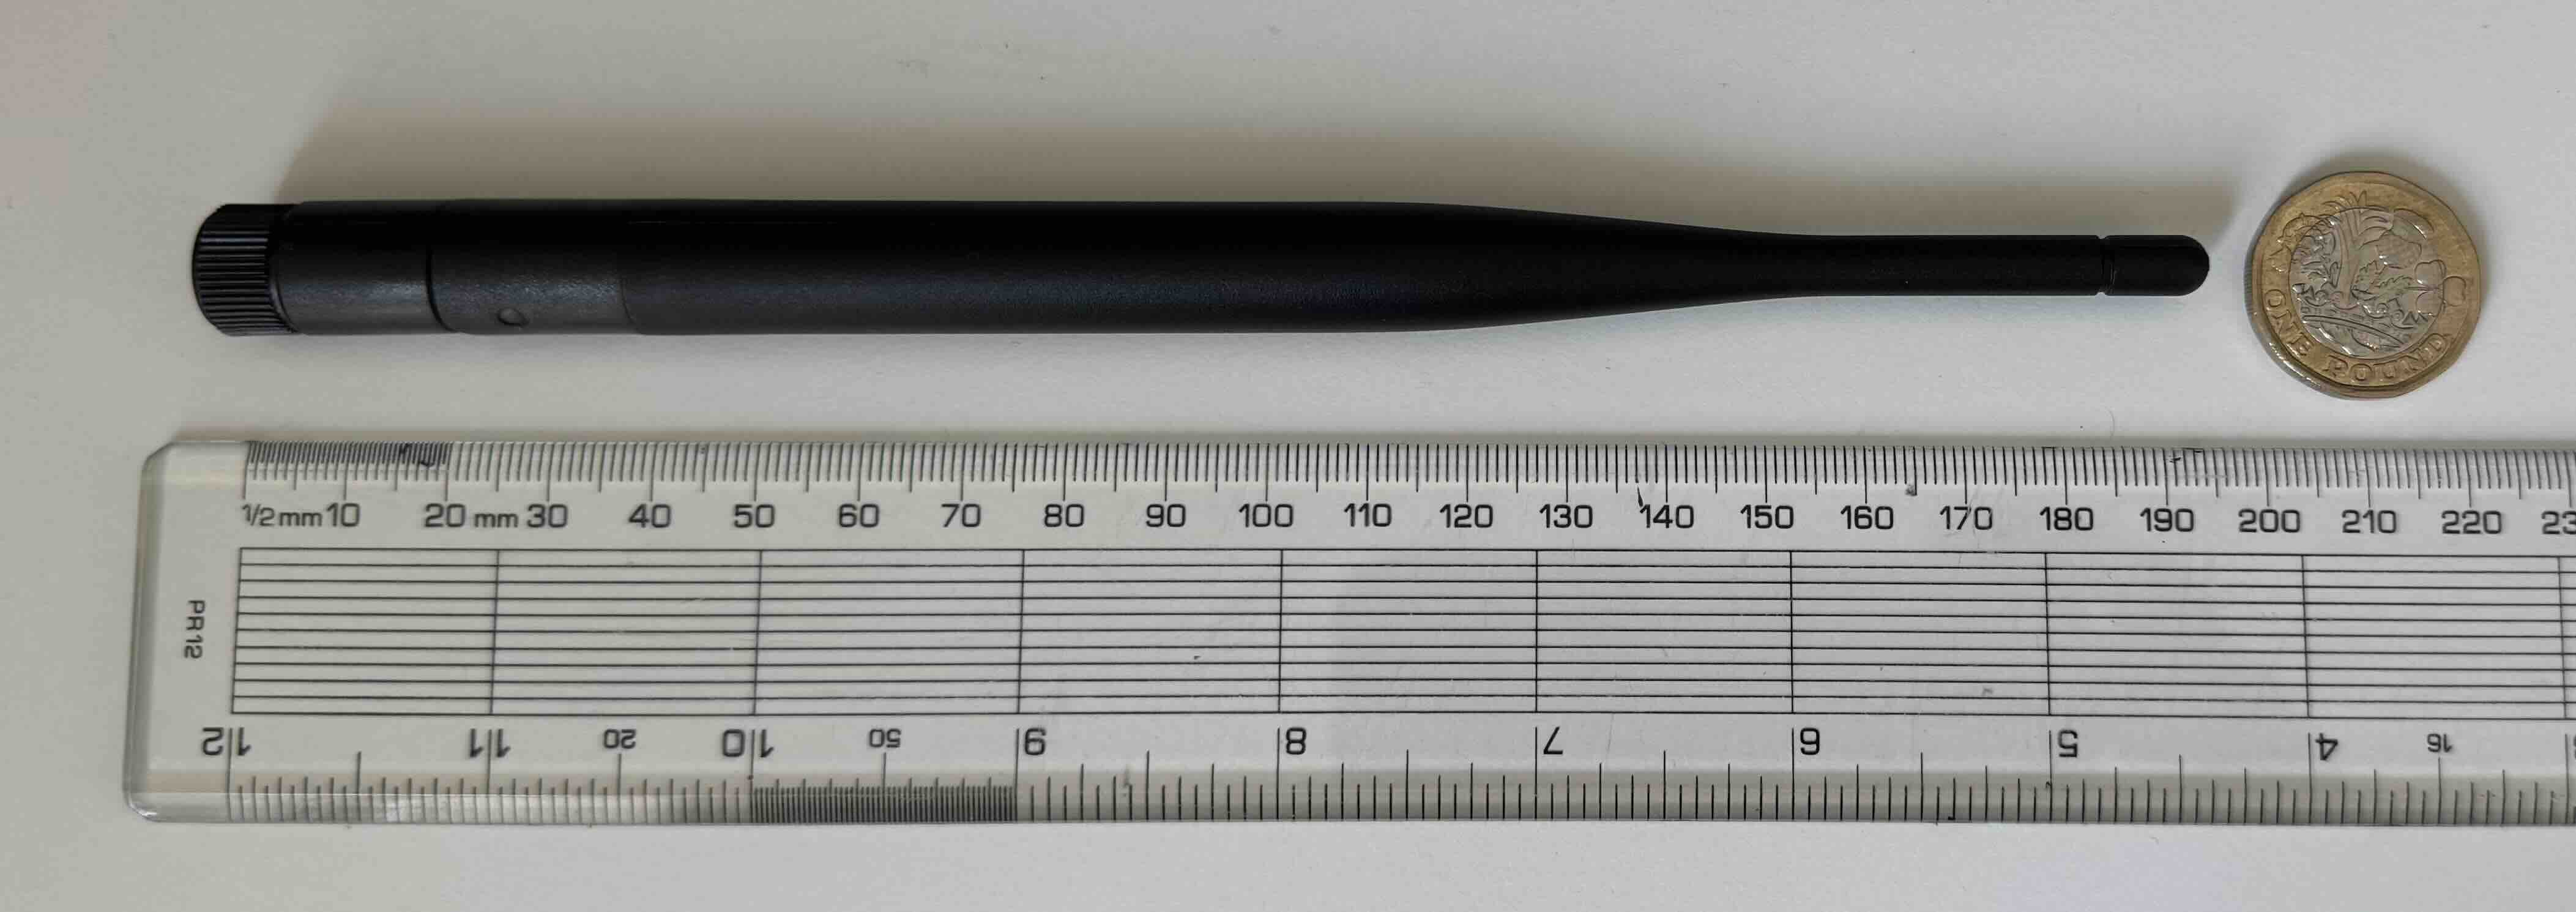
\includegraphics[width=0.8\textwidth]{contents/part-2/fig2/good-antenna.jpg}
    \caption{iLabs whip style LoRa antenna (868mhz)}
    \label{fig:good-antenna}
\end{figure}

\subsubsection{Powering the node}

To allow for continuous operation away from power sources, I attached a 6W
Monocrystalline Silicon Solar Panel (Figure~\ref{fig:solar-module})to each of
the nodes. I also installed a solar power management module
(Figure~\ref{fig:solar-module}) onto the Challengers. This module moderates the
output from the solar panels which is at too high a voltage to directly power
the nodes. It also incorporates a battery that charges from the solar panel
output and provides power to the nodes when the solar power is not available.

\begin{figure}[H]
    \centering
    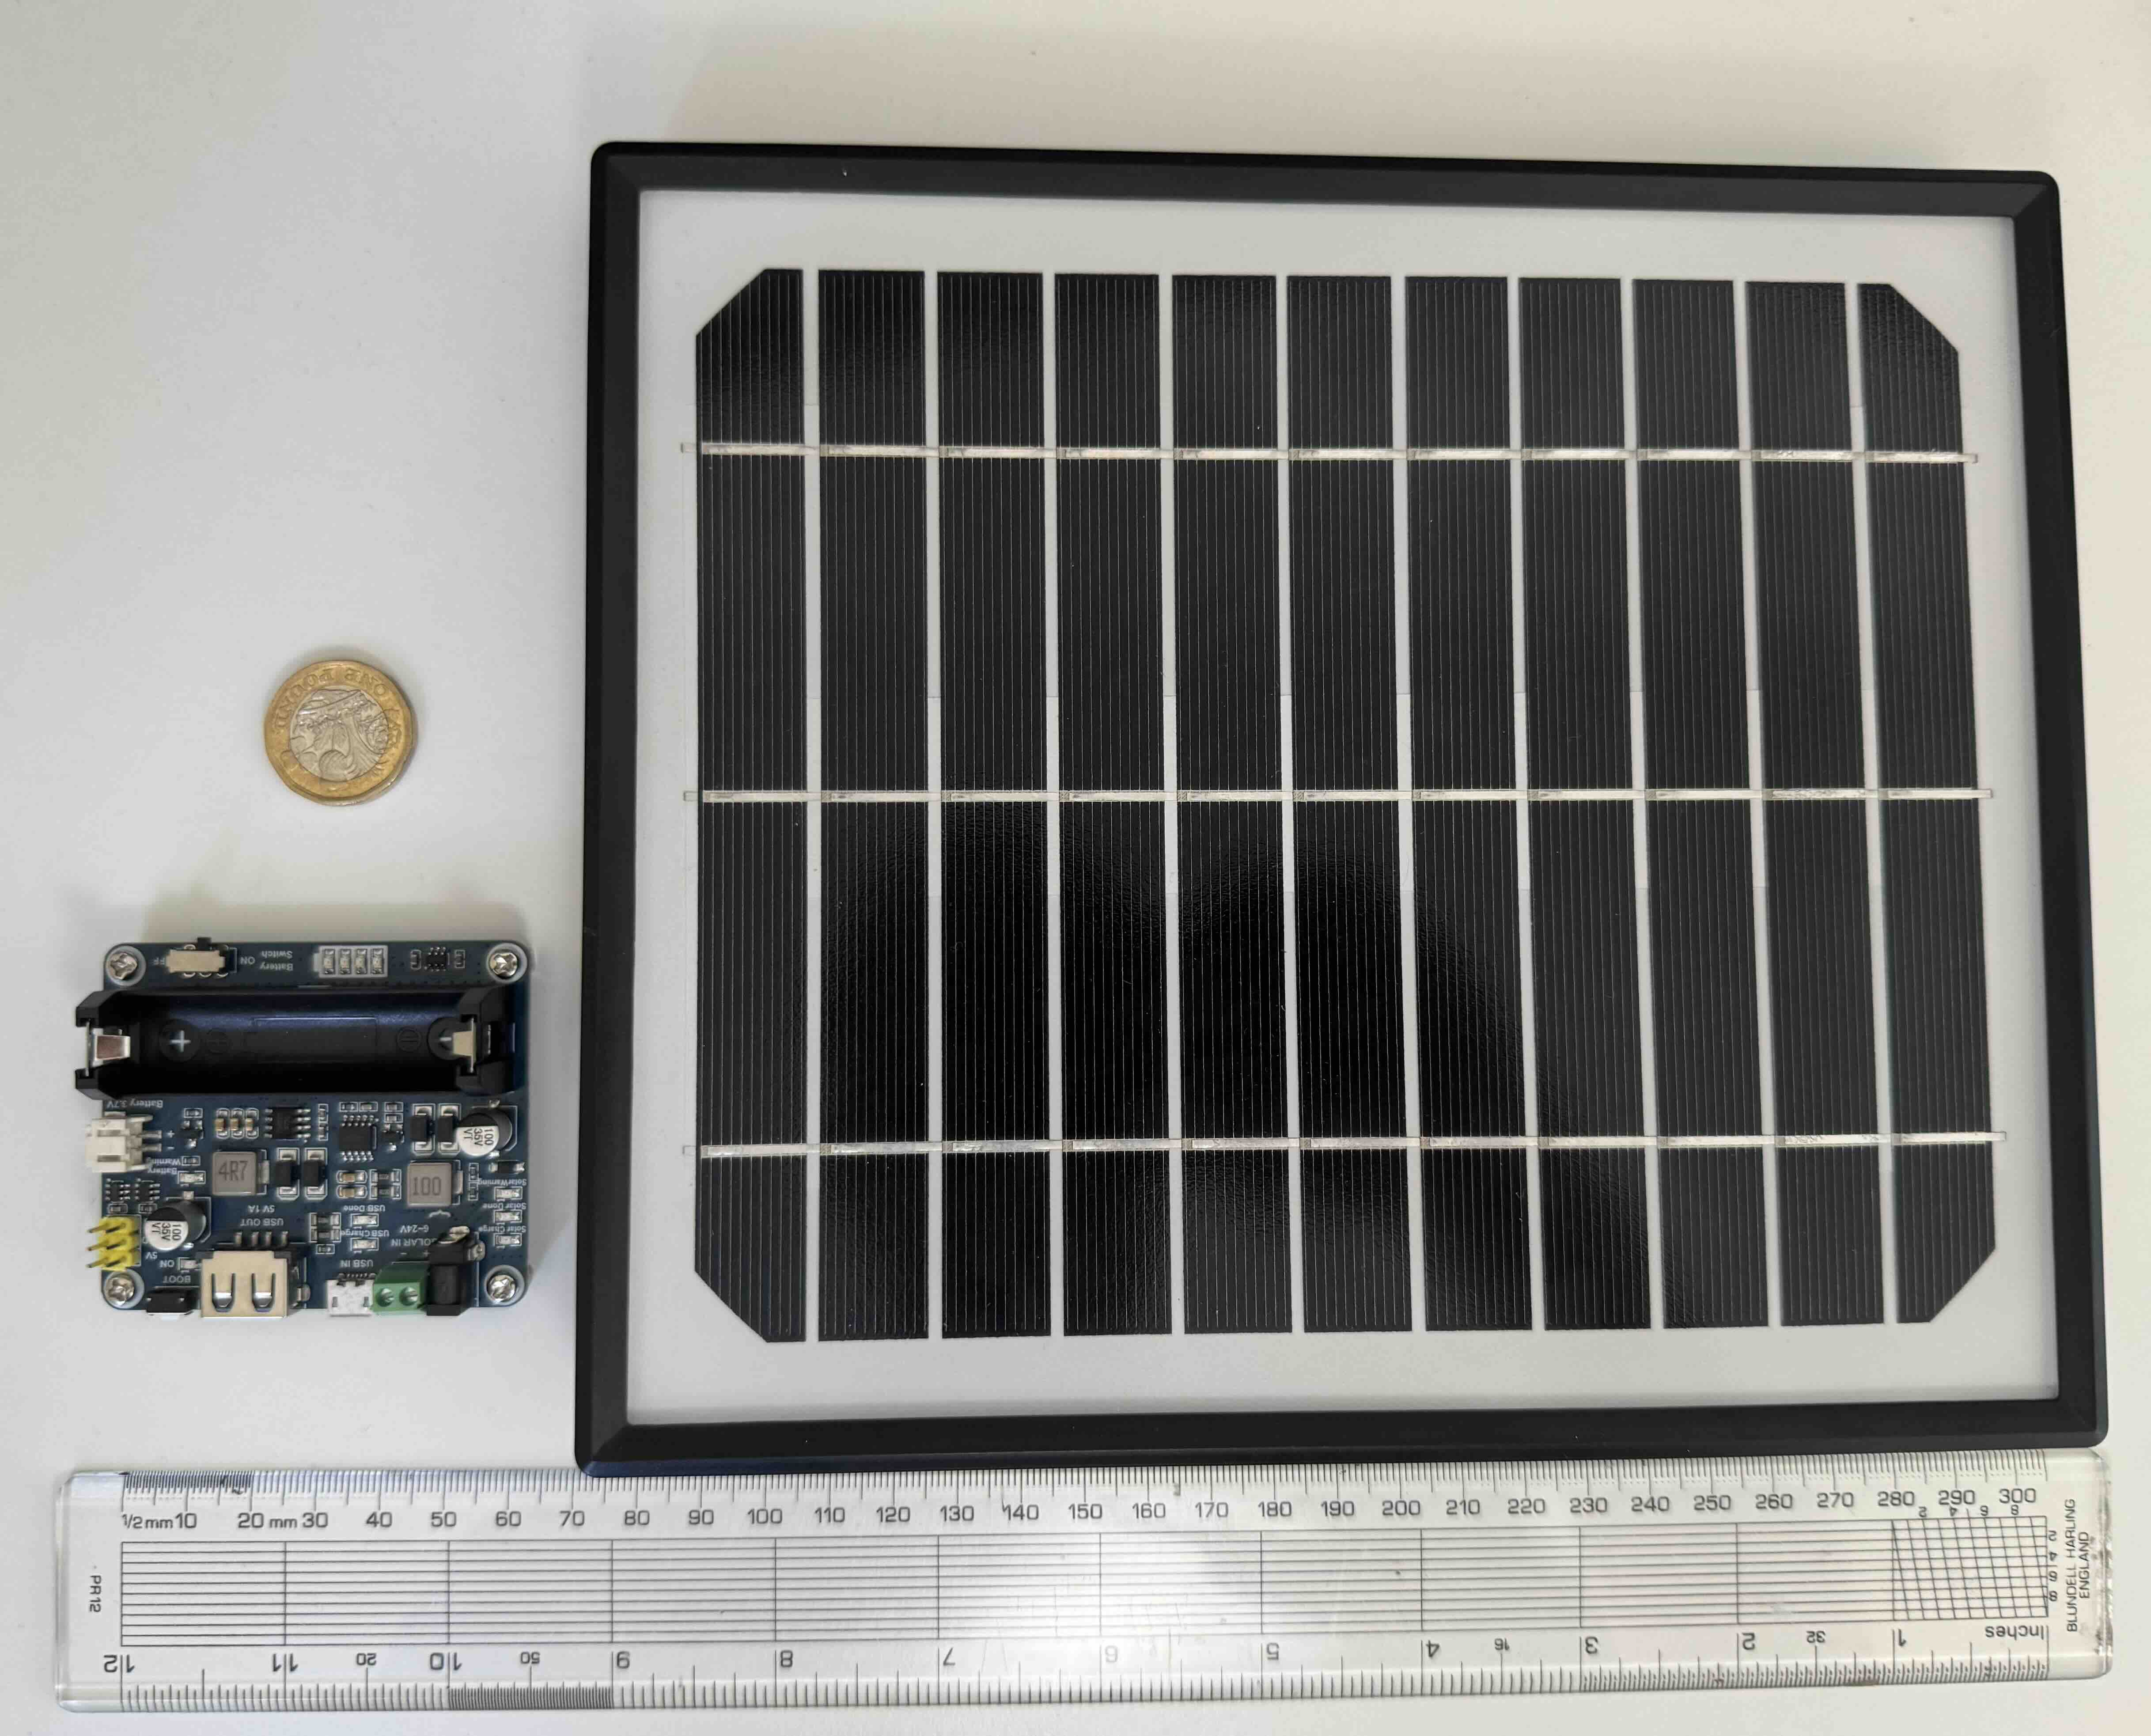
\includegraphics[width=0.5\textwidth]{contents/part-2/fig2/solar-panel-manager.jpg}
    \caption{Waveshare solar power management module (left), solar panel (right)}
    \label{fig:solar-module}
\end{figure}

\subsubsection{Sensor selection} \label{sec:sensor-selection}

\paragraph{Temperature and humidity sensor}

I used a DHT11 temperature/humidity sensor (Figure~\ref{fig:dht11}) for each
sensor node to provide basic readings. It was chosen for it's low cost,
availability and compatibility with both the RP2040 Challenger and CircuitPython
(via libraries). The sensor can be connected to the microcontroller using a
single GPIO pin as well as the usual power and ground pin.

\begin{figure}[H]
    \centering
    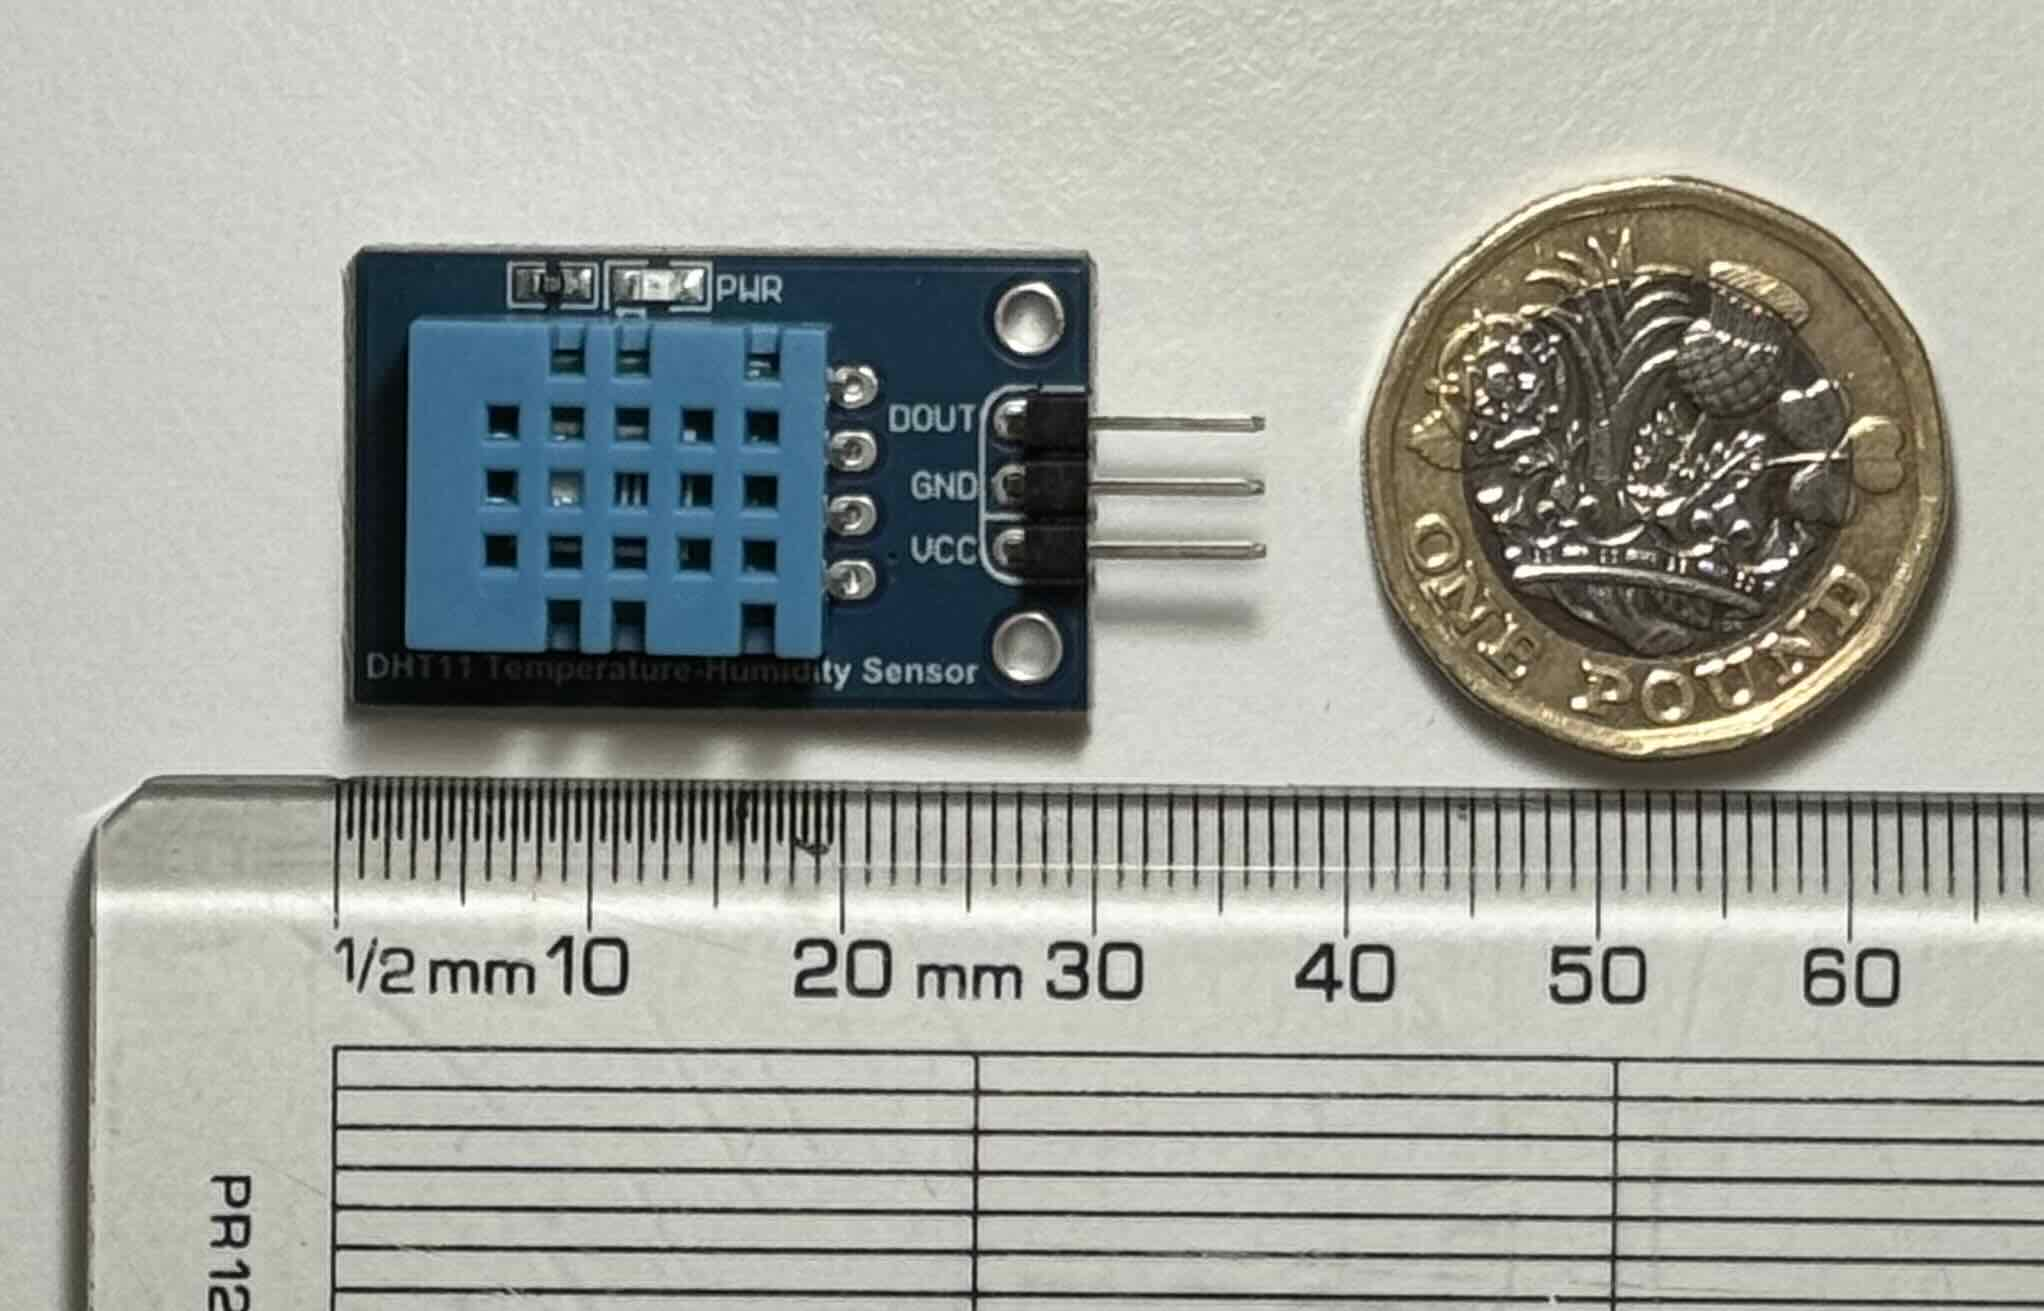
\includegraphics[width=0.7\textwidth]{contents/part-2/fig2/dht11.jpg}
    \caption{Waveshare DHT11 temperature/humidity sensor}
    \label{fig:dht11}
\end{figure}

\paragraph{Soil moisture sensor}

The main choice between soil moisture sensors is whether to use a capacitative
or resistive style sensor. In a resistance sensor the diodes must be bare plated
metal in order for resistance between each diode to be measured. However the
disadvantage of this is that bare metal corrodes in the presence of water, and
corrosion affects the accuracy of the sensor.  The benefit of capacitative
sensors is that the diodes are covered by a protective layer making them much
less susceptible to corrosion. For this reason I chose a capacitive sensor
(Figure~\ref{fig:soil-sensor}).


\begin{figure}[H]
    \centering
    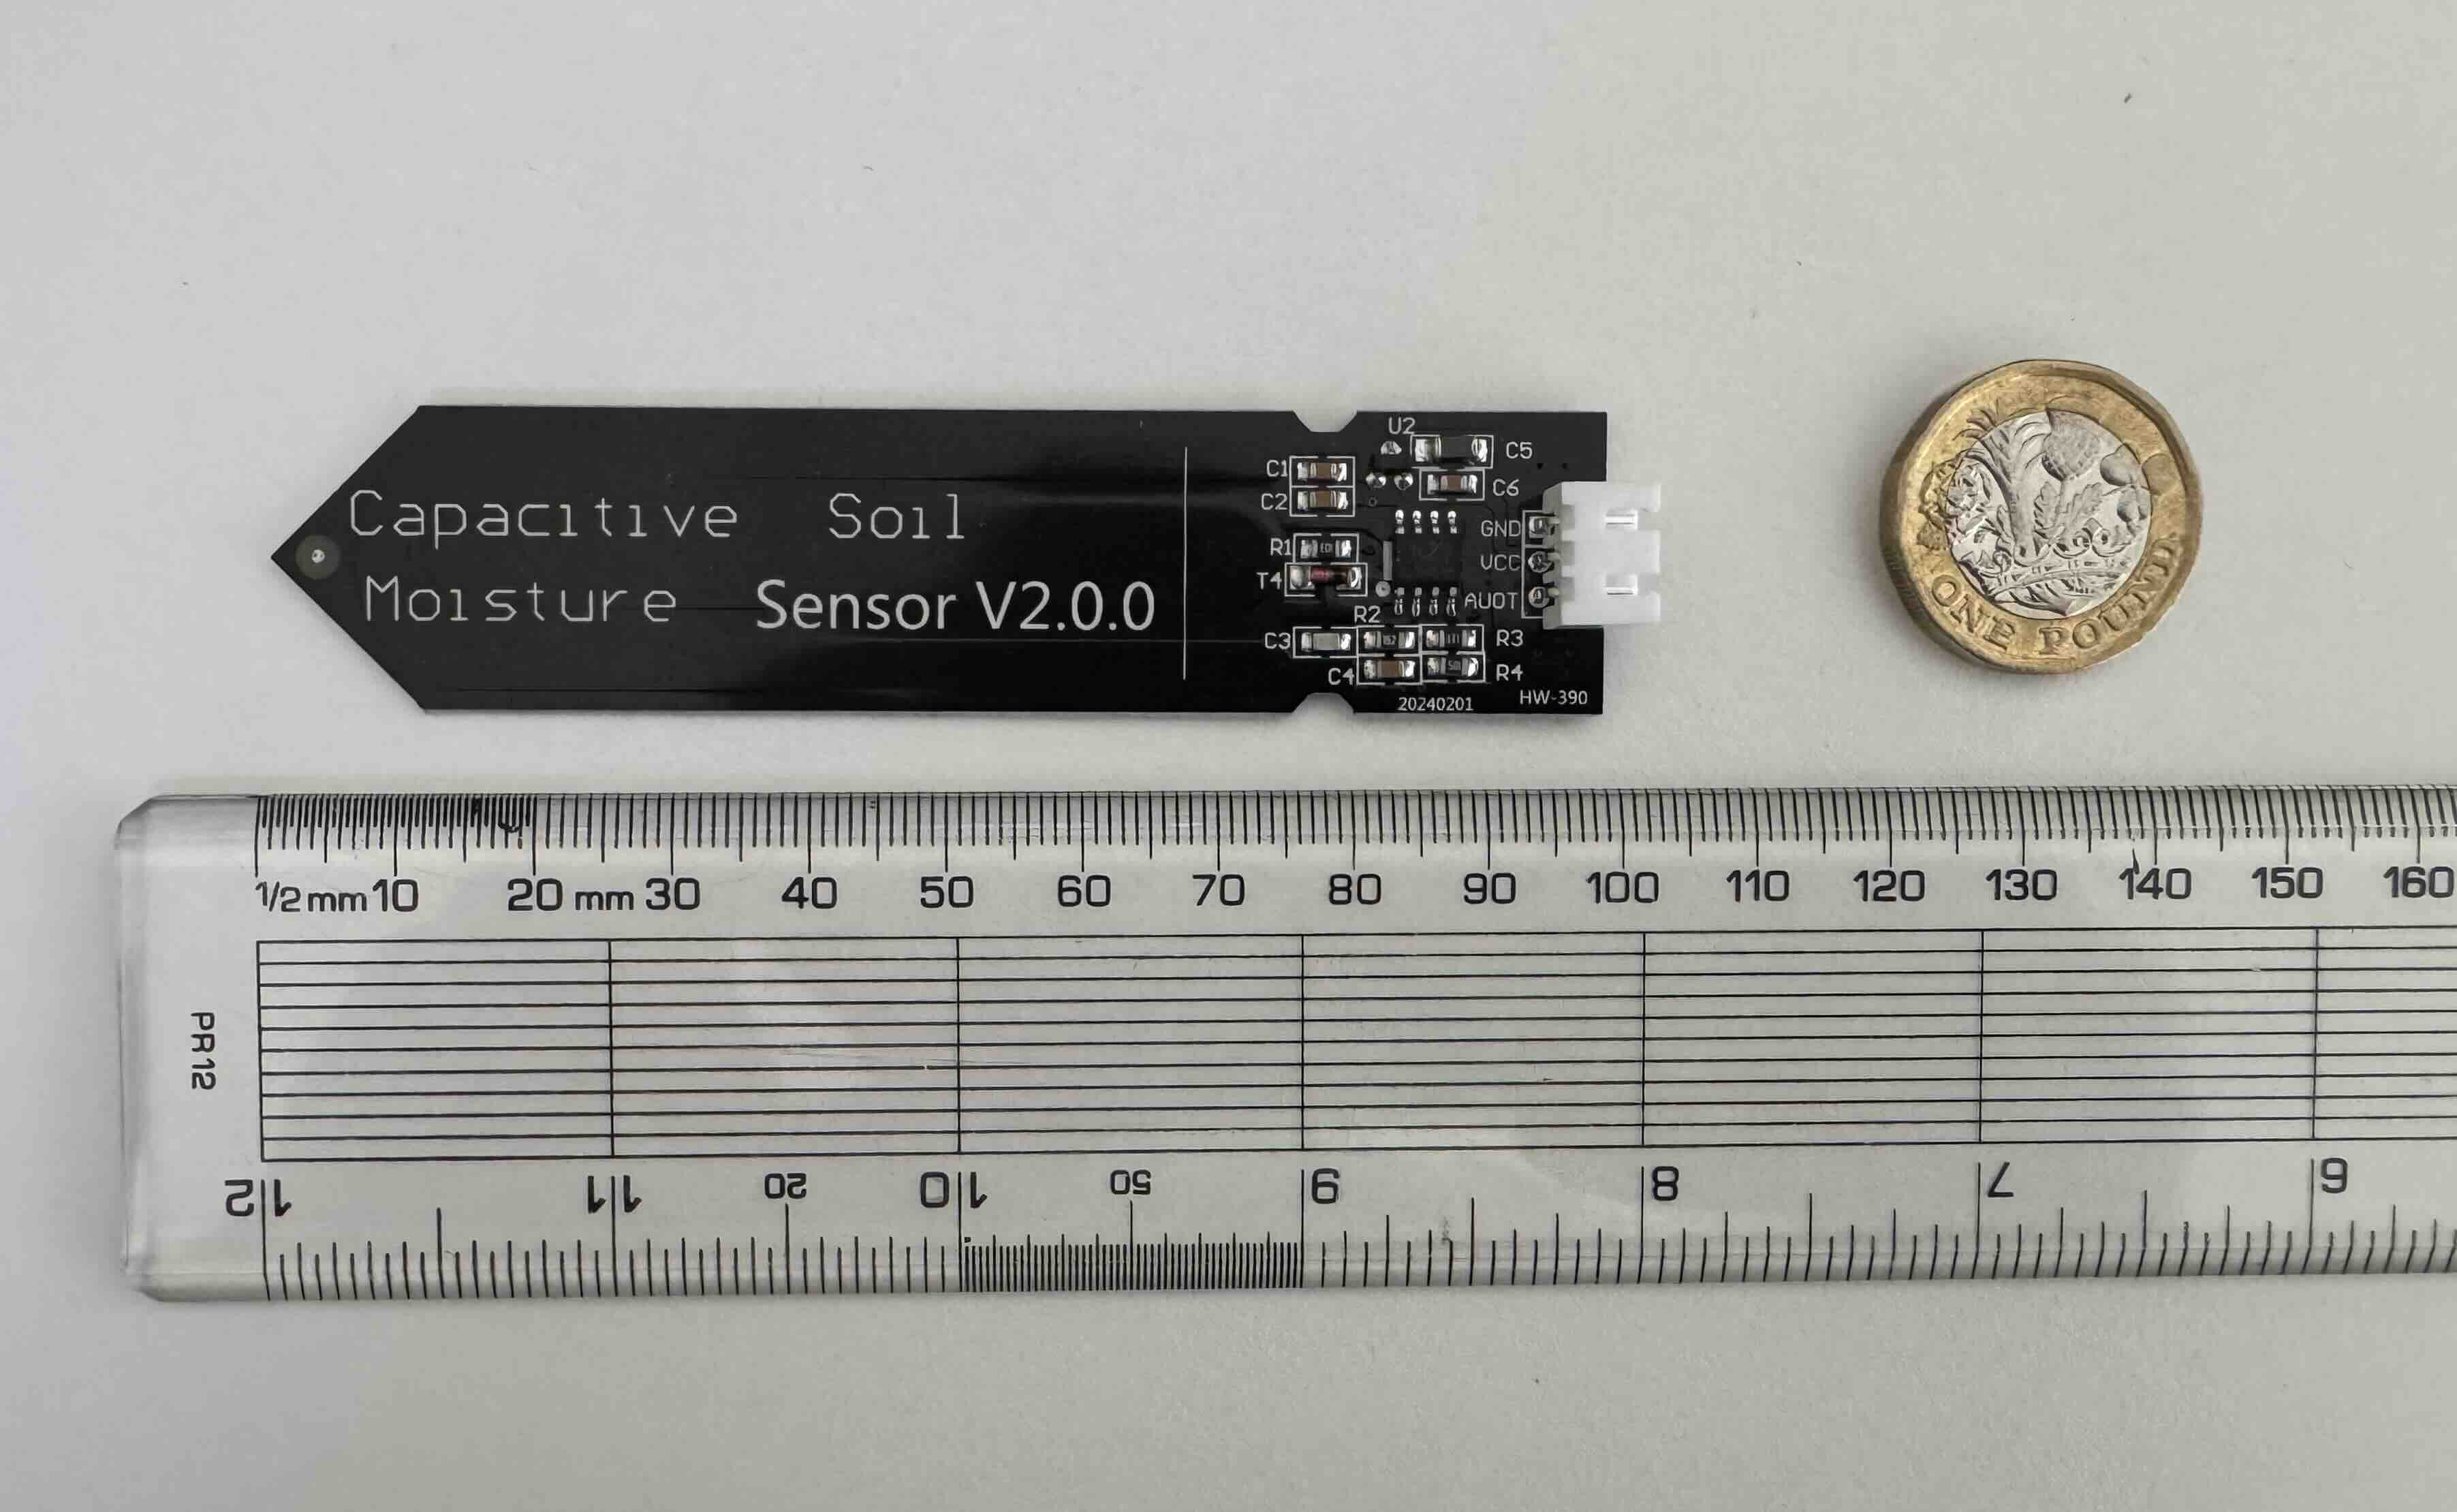
\includegraphics[width=0.7\textwidth]{contents/part-2/fig2/soil-sensor.jpg}
    \caption{The Pi Hut capacitive soil moisture sensor}
    \label{fig:soil-sensor}
\end{figure}

\paragraph{Wind speed sensor (Anemometer)}\label{sec:anemometer}

The anemometer chosen (Figure~\ref{fig:wind-sensor}) was the DFROBOT wind speed
sensor. It balances value with construction quality as unlike many other cup
style sensors this is made of metal and rated for outdoor use. When I chose this
component I was unaware that the RS485 serial communication protocol that the
sensor used was not compatible with the Challengers UART protocol. Fortunately,
I was able to purchase an RS485 to UART serial converter that allowed the
devices to communicate.

\begin{figure}[H]
    \centering
    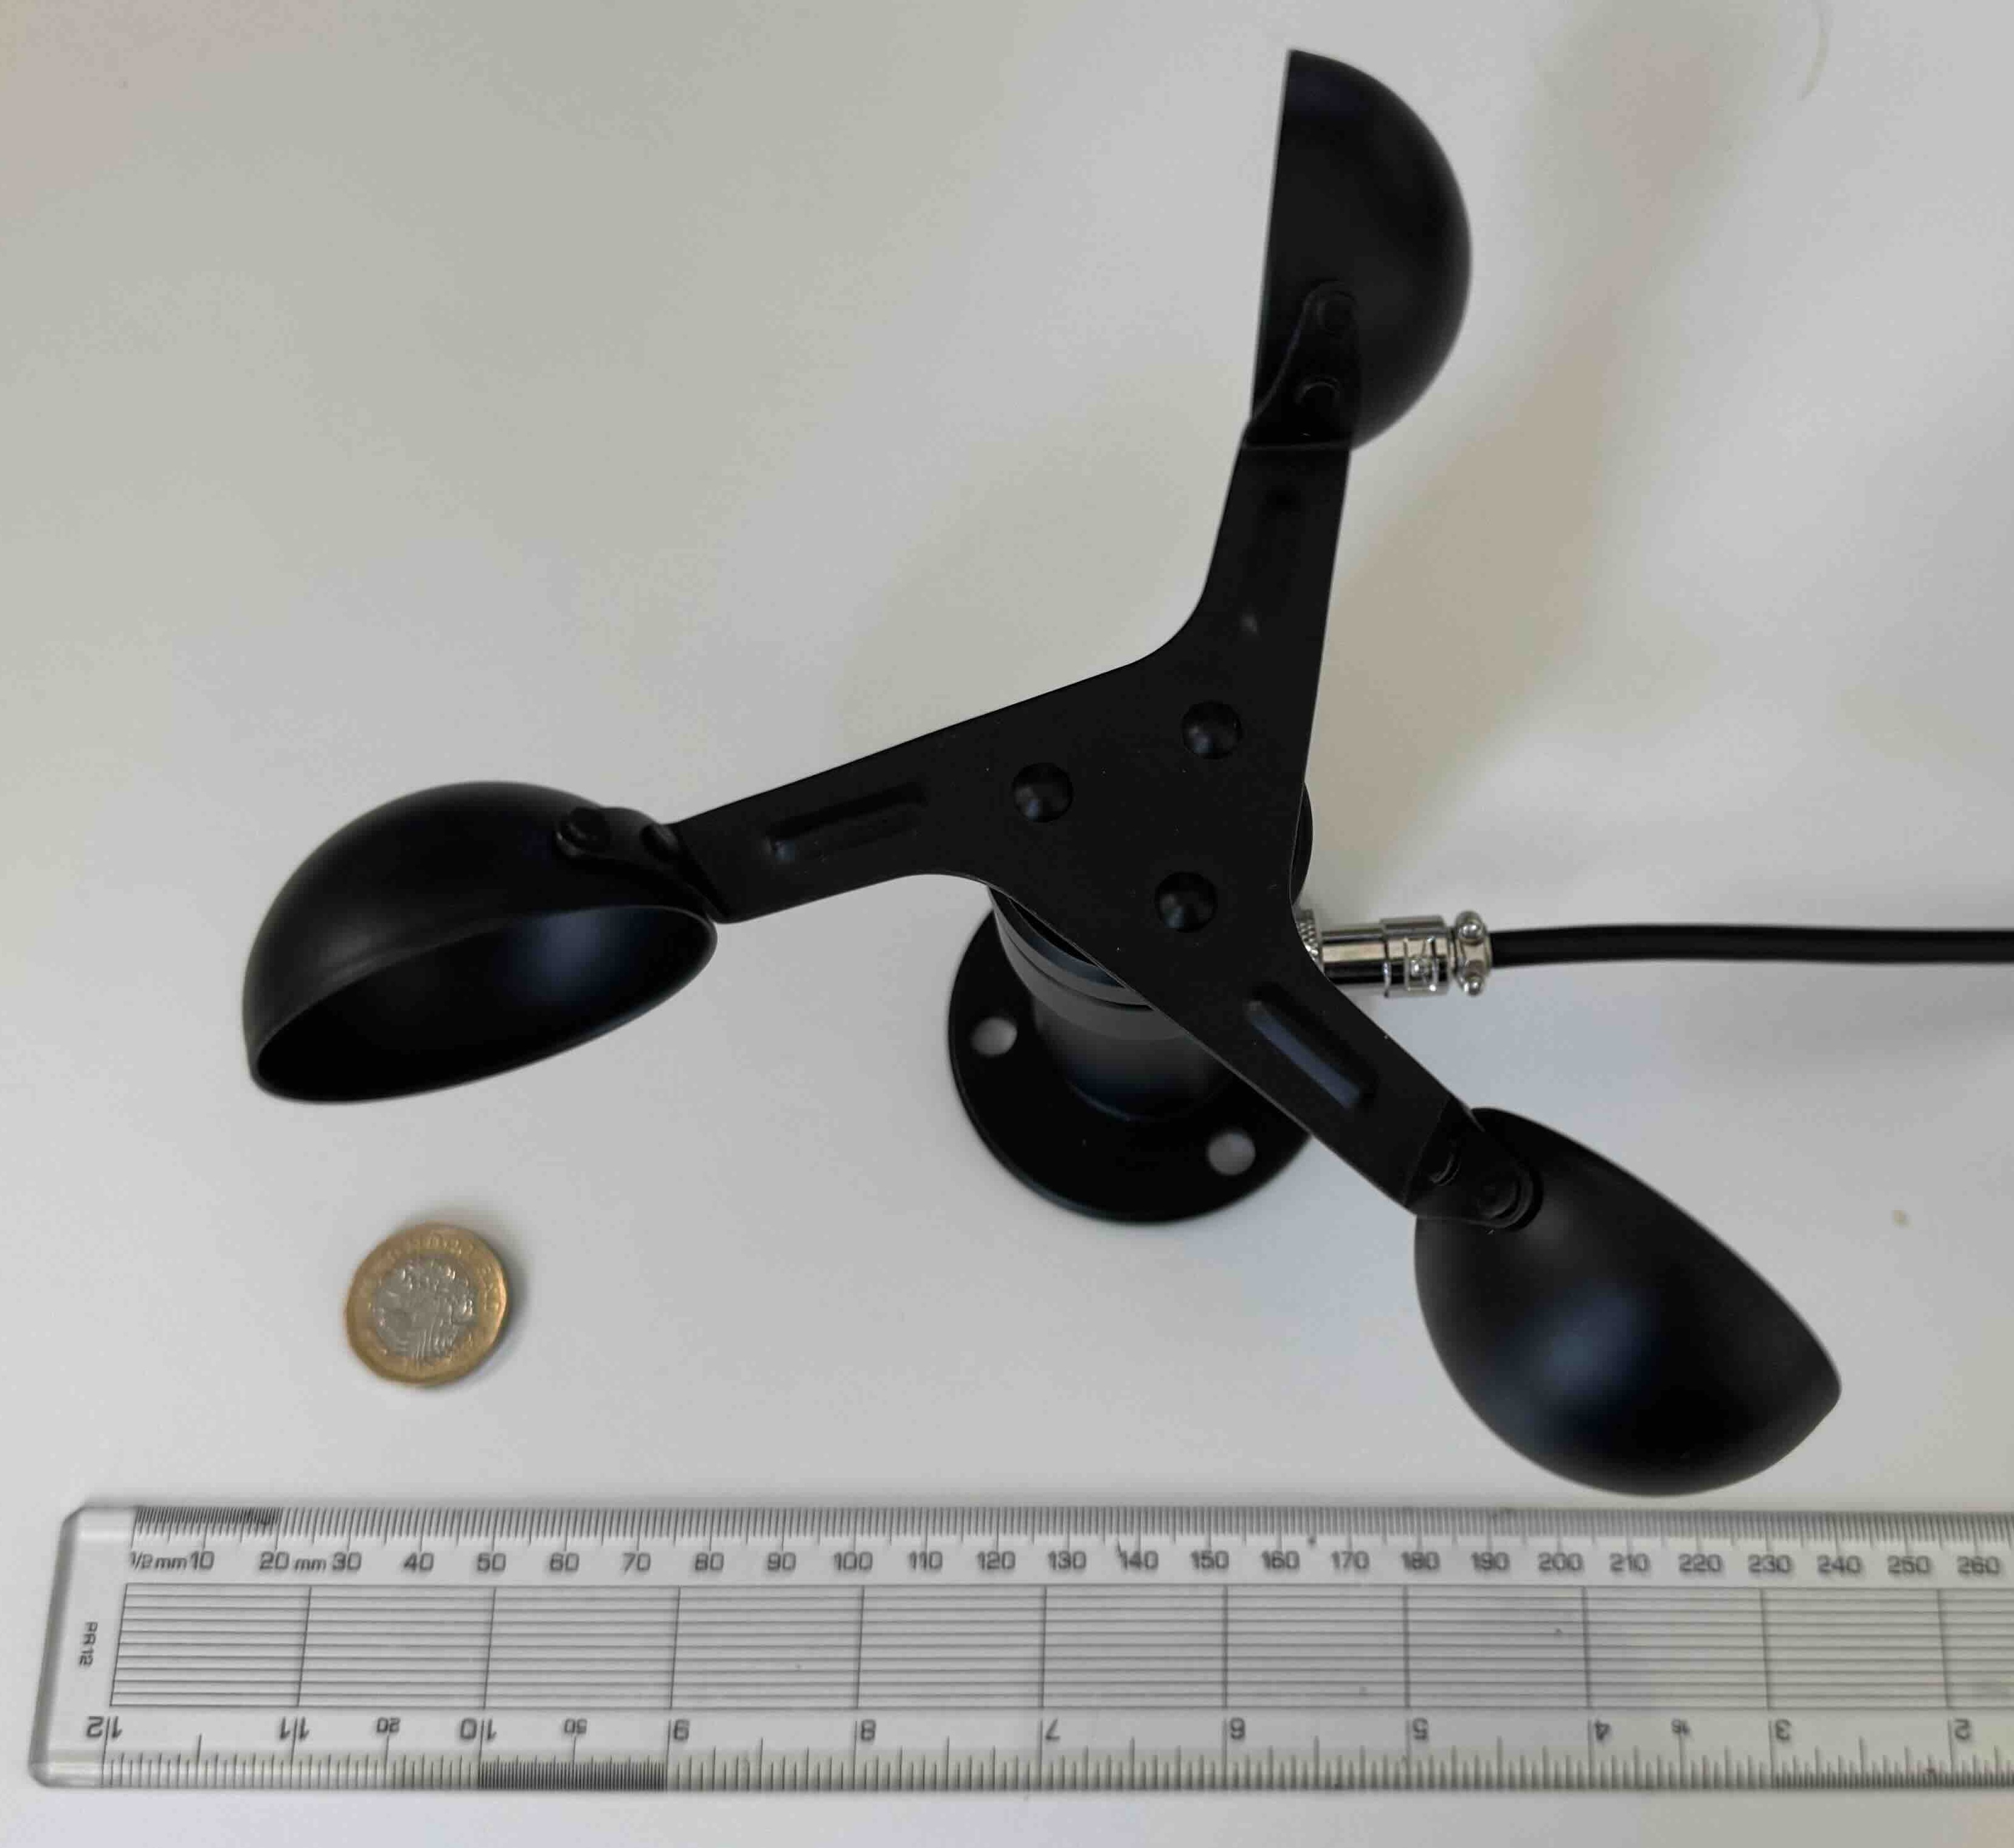
\includegraphics[width=0.5\textwidth]{contents/part-2/fig2/wind-sensor.jpg}
    \caption{DFROBOT wind speed sensor}
    \label{fig:wind-sensor}
\end{figure}

A second issue was that the anemometer needed a 7V-24V input voltage to take
readings while the maximum voltage the Challenger can provide was 5V. To remedy
this I bought a 9V step up converter to boost the Challenger's voltage to the
required level.

\subsection{Gateway}

The components of the gateway consisted of a Challenger RP2040 with a whip
antenna. The board was connected to a Raspberry Pi 5 with 8GB of memory and an
onboard Wi-Fi radio. (Figure~\ref{fig:raspberry-pi}). This Raspberry Pi was
significantly more powerful than was needed but it was already available from
the university for use for this project. The Challenger receives and decodes
messages from the repeater. The Raspberry Pi reads the decoded LoRa message from
the serial output and then sends a POST response to the backend API which
inserts the data into a SQL database.

\begin{figure}[H]
    \centering
    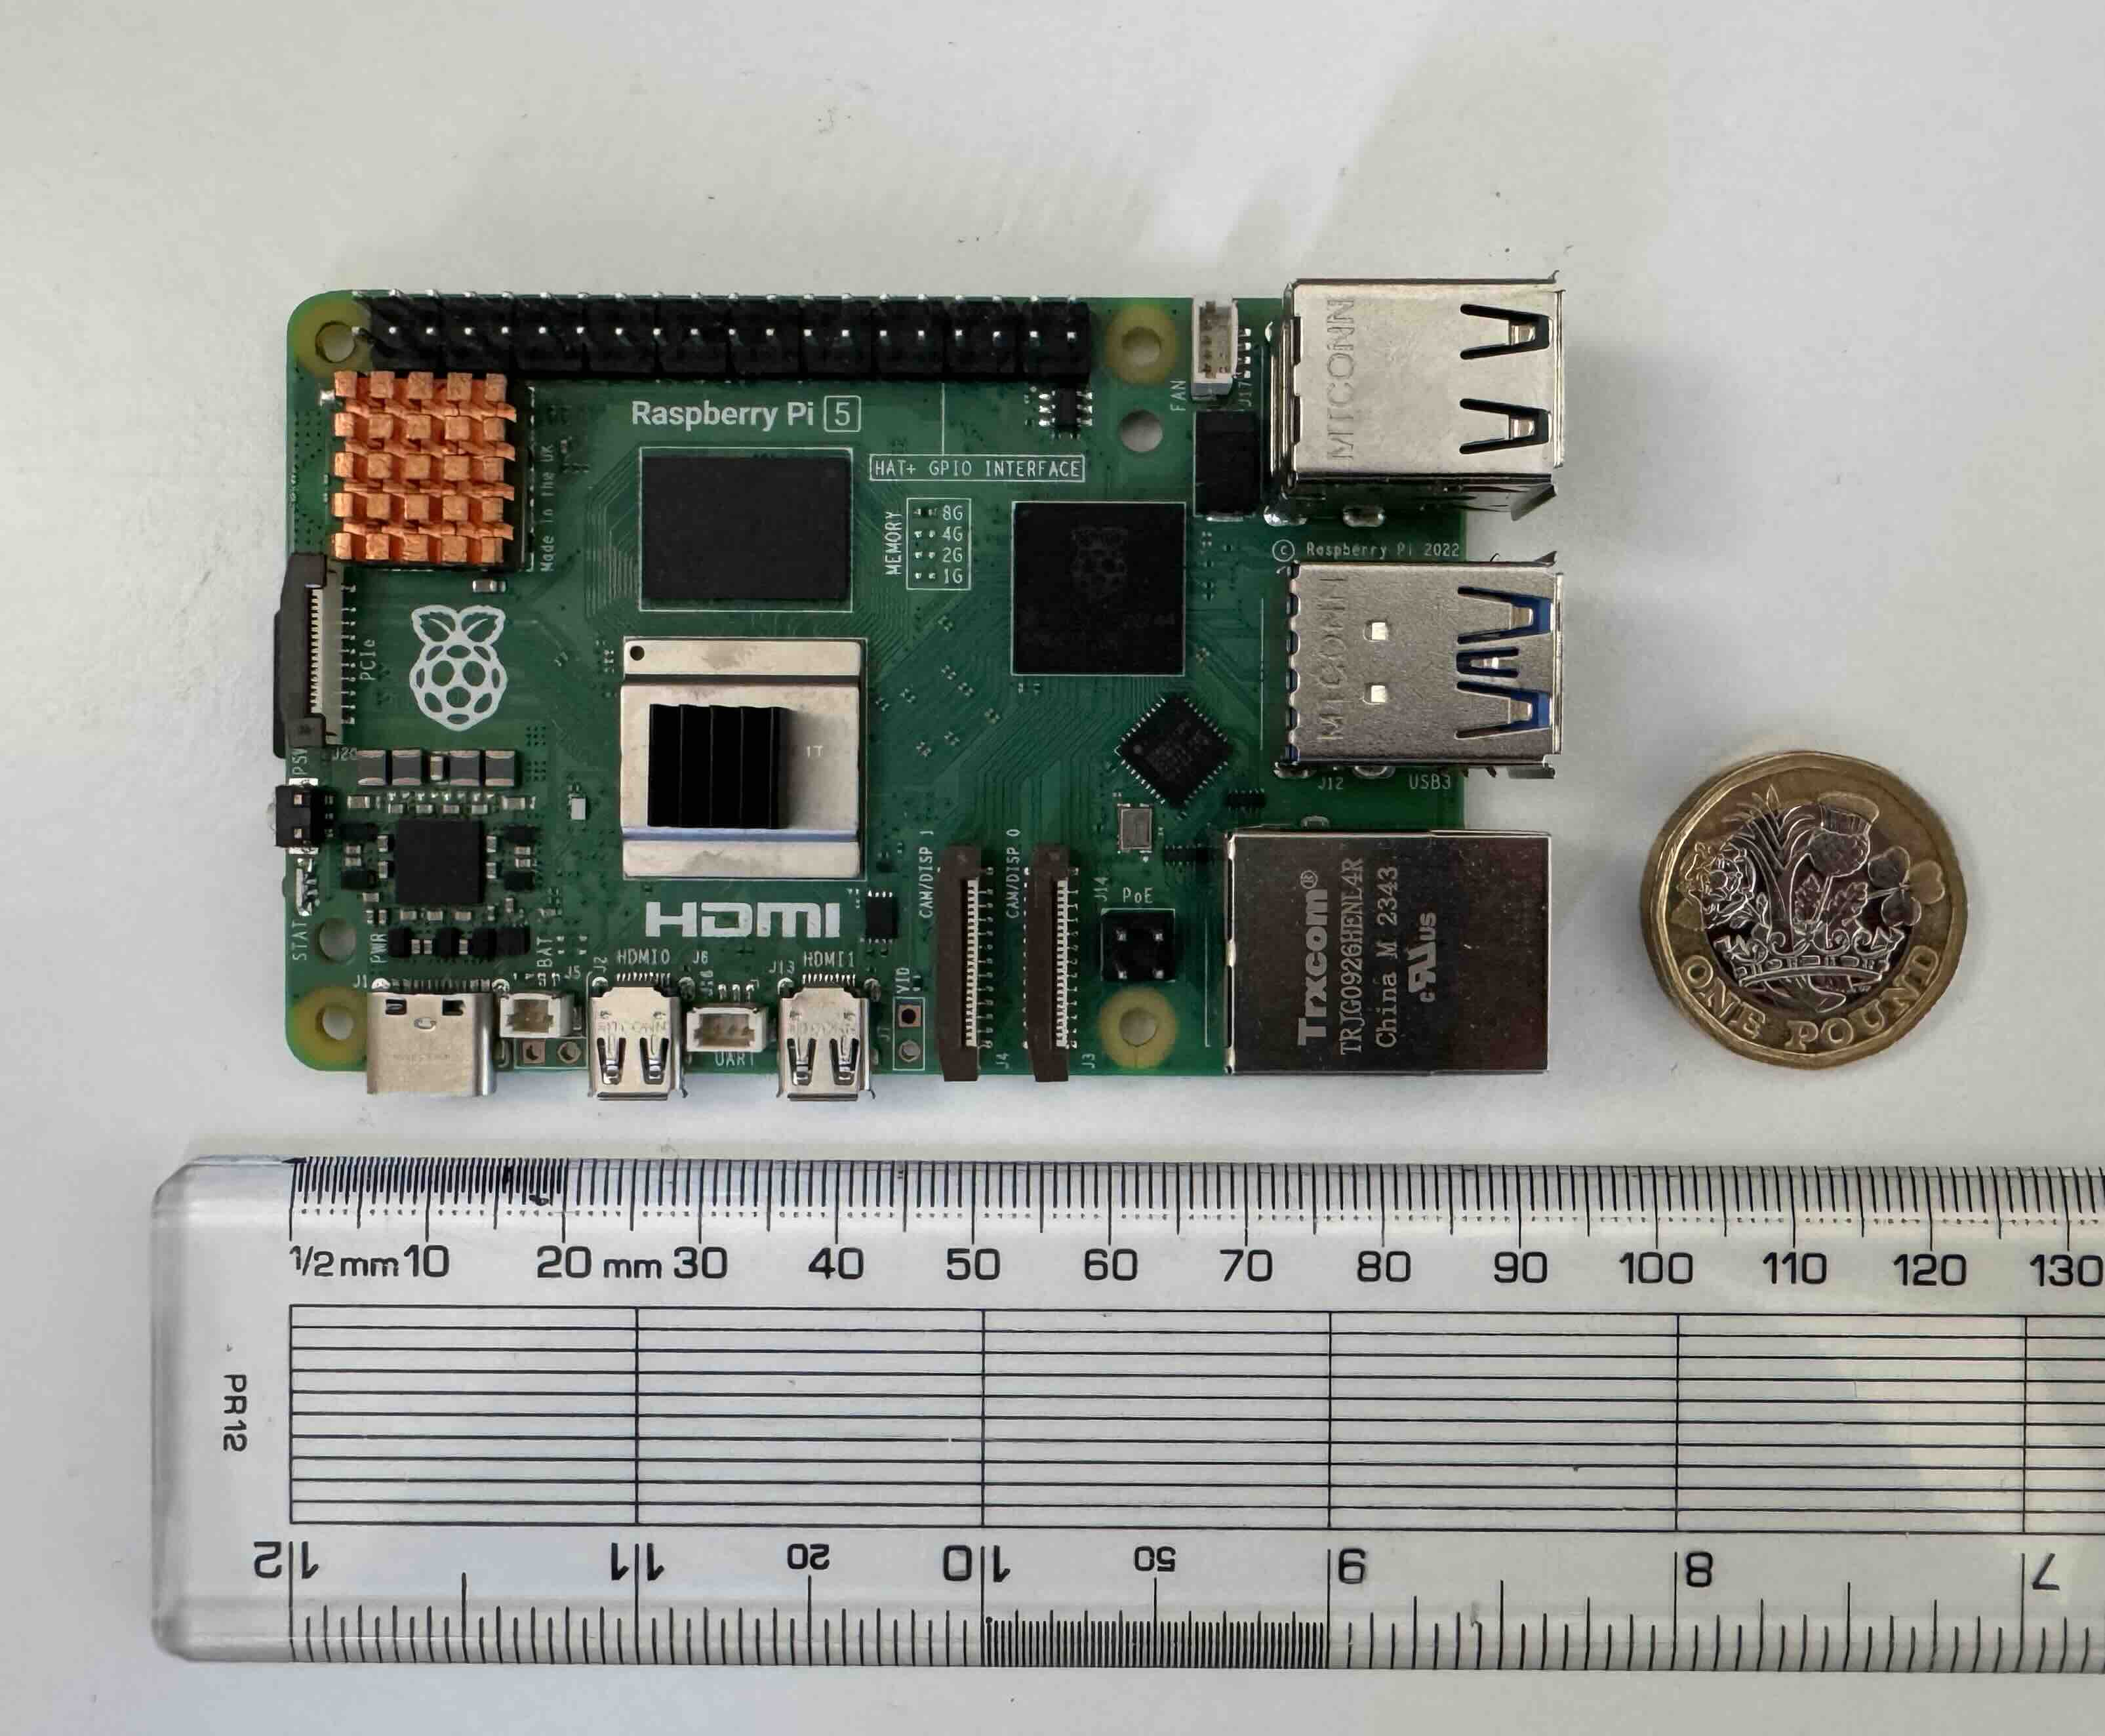
\includegraphics[width=0.4\textwidth]{contents/part-2/fig2/raspberry-pi.jpg}
    \caption{Raspberry Pi 5 (8GB)}
    \label{fig:raspberry-pi}
\end{figure}

